% Created 2021-04-08 Thu 11:31
% Intended LaTeX compiler: pdflatex

  \documentclass[english]{article}
  \usepackage[T1, T2A]{fontenc}
\usepackage[lutf8]{luainputenc}
\usepackage[english, russian]{babel}
\usepackage{minted}
\usepackage{graphicx}
\usepackage{longtable}
\usepackage{hyperref}
\usepackage{xcolor}
\usepackage{natbib}
\usepackage{amssymb}
\usepackage{stmaryrd}
\usepackage{amsmath}
\usepackage{caption}
\usepackage{mathtools}
\usepackage{amsthm}
\usepackage{tikz}
\usepackage{grffile}
\usepackage{extarrows}
\usepackage{wrapfig}
\usepackage{algorithm}
\usepackage{algorithmic}
\usepackage{lipsum}
\usepackage{rotating}
\usepackage{placeins}
\usepackage[normalem]{ulem}
\usepackage{amsmath}
\usepackage{textcomp}
\usepackage{capt-of}
  
  \usepackage{geometry}
  \geometry{a4paper,left=2.5cm,top=2cm,right=2.5cm,bottom=2cm,marginparsep=7pt, marginparwidth=.6in}
   \usepackage{hyperref}
 \hypersetup{
     colorlinks=true,
     linkcolor=blue,
     filecolor=orange,
     citecolor=black,      
     urlcolor=cyan,
     }

\usetikzlibrary{decorations.markings}
\usetikzlibrary{cd}
\usetikzlibrary{patterns}
\usetikzlibrary{automata, arrows}

\newcommand\addtag{\refstepcounter{equation}\tag{\theequation}}
\newcommand{\eqrefoffset}[1]{\addtocounter{equation}{-#1}(\arabic{equation}\addtocounter{equation}{#1})}


\newcommand{\R}{\mathbb{R}}
\renewcommand{\C}{\mathbb{C}}
\newcommand{\N}{\mathbb{N}}
\newcommand{\A}{\mathfrak{A}}
\newcommand{\rank}{\mathop{\rm rank}\nolimits}
\newcommand{\const}{\var{const}}
\newcommand{\grad}{\mathop{\rm grad}\nolimits}

\newcommand{\todo}{{\color{red}\fbox{\text{Доделать}}}}
\newcommand{\fixme}{{\color{red}\fbox{\text{Исправить}}}}

\newcounter{propertycnt}
\setcounter{propertycnt}{1}
\newcommand{\beginproperty}{\setcounter{propertycnt}{1}}

\theoremstyle{plain}
\newtheorem{propertyinner}{Свойство}
\newenvironment{property}{
  \renewcommand\thepropertyinner{\arabic{propertycnt}}
  \propertyinner
}{\endpropertyinner\stepcounter{propertycnt}}
\newtheorem{axiom}{Аксиома}
\newtheorem{lemma}{Лемма}
\newtheorem{manuallemmainner}{Лемма}
\newenvironment{manuallemma}[1]{%
  \renewcommand\themanuallemmainner{#1}%
  \manuallemmainner
}{\endmanuallemmainner}

\theoremstyle{remark}
\newtheorem*{remark}{Примечание}
\newtheorem*{solution}{Решение}
\newtheorem{corollary}{Следствие}[theorem]
\newtheorem*{examp}{Пример}
\newtheorem*{observation}{Наблюдение}

\theoremstyle{definition}
\newtheorem{task}{Задача}
\newtheorem{theorem}{Теорема}[section]
\newtheorem*{definition}{Определение}
\newtheorem*{symb}{Обозначение}
\newtheorem{manualtheoreminner}{Теорема}
\newenvironment{manualtheorem}[1]{%
  \renewcommand\themanualtheoreminner{#1}%
  \manualtheoreminner
}{\endmanualtheoreminner}
\captionsetup{justification=centering,margin=2cm}
\newenvironment{colored}[1]{\color{#1}}{}

\tikzset{->-/.style={decoration={
  markings,
  mark=at position .5 with {\arrow{>}}},postaction={decorate}}}
\makeatletter
\newcommand*{\relrelbarsep}{.386ex}
\newcommand*{\relrelbar}{%
  \mathrel{%
    \mathpalette\@relrelbar\relrelbarsep
  }%
}
\newcommand*{\@relrelbar}[2]{%
  \raise#2\hbox to 0pt{$\m@th#1\relbar$\hss}%
  \lower#2\hbox{$\m@th#1\relbar$}%
}
\providecommand*{\rightrightarrowsfill@}{%
  \arrowfill@\relrelbar\relrelbar\rightrightarrows
}
\providecommand*{\leftleftarrowsfill@}{%
  \arrowfill@\leftleftarrows\relrelbar\relrelbar
}
\providecommand*{\xrightrightarrows}[2][]{%
  \ext@arrow 0359\rightrightarrowsfill@{#1}{#2}%
}
\providecommand*{\xleftleftarrows}[2][]{%
  \ext@arrow 3095\leftleftarrowsfill@{#1}{#2}%
}
\makeatother

\newenvironment{rualgo}[1][]
  {\begin{algorithm}[#1]
     \selectlanguage{russian}%
     \floatname{algorithm}{Алгоритм}%
     \renewcommand{\algorithmicif}{{\color{red}\textbf{если}}}%
     \renewcommand{\algorithmicthen}{{\color{red}\textbf{тогда}}}%
     \renewcommand{\algorithmicelse}{{\color{red}\textbf{иначе}}}%
     \renewcommand{\algorithmicend}{{\color{red}\textbf{конец}}}%
     \renewcommand{\algorithmicfor}{{\color{red}\textbf{для}}}%
     \renewcommand{\algorithmicto}{{\color{red}\textbf{до}}}%
     \renewcommand{\algorithmicdo}{{\color{red}\textbf{делать}}}%
     \renewcommand{\algorithmicwhile}{{\color{red}\textbf{пока}}}%
     \renewcommand{\algorithmicrepeat}{{\color{red}\textbf{повторять}}}%
     \renewcommand{\algorithmicuntil}{{\color{red}\textbf{до тех пор пока}}}%
     \renewcommand{\algorithmicloop}{{\color{red}\textbf{повторять}}}%
     \renewcommand{\algorithmicnot}{{\color{blue}\textbf{не}}}%
     \renewcommand{\algorithmicand}{{\color{blue}\textbf{и}}}%
     \renewcommand{\algorithmicor}{{\color{blue}\textbf{или}}}%
     \renewcommand{\algorithmicrequire}{{\color{blue}\textbf{Предусловие}}}%
     \renewcommand{\algorithmicrensure}{{\color{blue}\textbf{Постусловие}}}%
     \renewcommand{\algorithmicrtrue}{{\color{blue}\textbf{истинна}}}%
     \renewcommand{\algorithmicrfalse}{{\color{blue}\textbf{ложь}}}%
     % Set other language requirements
  }
  {\end{algorithm}}
\author{Ilya Yaroshevskiy}
\date{\today}
\title{Практика 8}
\hypersetup{
 pdfauthor={Ilya Yaroshevskiy},
 pdftitle={Практика 8},
 pdfkeywords={},
 pdfsubject={},
 pdfcreator={Emacs 28.0.50 (Org mode 9.4.4)}, 
 pdflang={English}}
\begin{document}

\maketitle
\tableofcontents

\begin{task}[4089]
\[ z = x^2 + y^2 \]
\end{task}
\begin{solution}
\[ r\sin\psi = r^2\cos^2\psi \Leftrightarrow r = \frac{\sin\psi}{\cos^2\psi} \]
\[ x = y \Leftrightarrow \varphi = \frac{\pi}{4} \]
\[ \cos \varphi = \sin\phi \]
\begin{itemize}
\item \(x = 1,\ r\cos\varphi\cos\psi = 1\)
\item \(r = 0,\ \psi = 0\)
\item \(y = 0,\ r\sin\varphi\cos\psi = 0,\ \phi = 0\)
\end{itemize}
\begin{figure}[htbp]
\centering
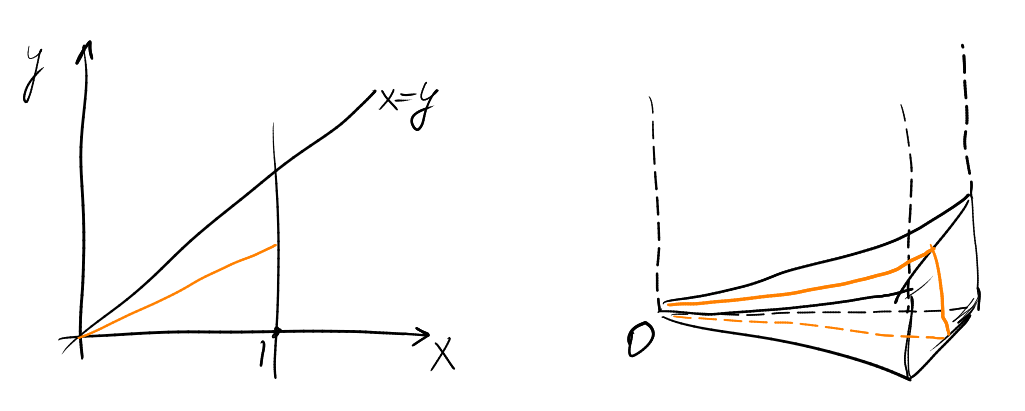
\includegraphics[scale=0.3]{8_1.png}
\caption{Фиксируем \(\varphi\)}
\end{figure}
\[ \int\limits_0^{\frac{\pi}{4}}d\varphi\int\limits_0^{\arctg\frac{1}{\cos\phi}} d\psi \int\limits_{\frac{\sin\psi}{\cos^2\psi}}^{\frac{1}{\cos\phi\cos\psi}} f(r)r^2\cos\psi\,dr \]
\end{solution}
Переходим в полярные координаты в плоскости \(xOy\):
\begin{itemize}
\item \(x = r\cos\varphi\)
\item \(y = r\sin\varphi\)
\item \(z = z\)
\end{itemize}
\[J = r\]
\begin{task}[4118.2]
\[ \sqrt[3]{\frac{x}{a}} + \sqrt[3]{\frac{y}{b}} + \sqrt[3]{\frac{z}{c}} = 1 \quad x, y, z \ge 0 \]
\end{task}
\begin{solution}
\-
\begin{itemize}
\item \(x = ar\cos^6\varphi\cos^6\psi\)
\item \(y = br\sin^6\varphi\cos^6\psi\)
\item \(z = cr \cos^6\psi\)
\end{itemize}
\[ r^{\frac{1}{3}} = 1 \]
\[ V = \iiint 1\,dx\,dy\,dz = \int_0^1 dr \int_0^{\frac{\pi}{2}} d\varphi \int_0^{\frac{\pi}{2}} abs\cdot 36\cdot \cos^5\phi\sin^5\phi\cos^{11?}\psi\sin^5\psi\]
\end{solution}
\begin{task}[4105]
\[ az = a^2 - x^2 - y^2 \]
\[ z = a - x - y \]
\[ x=0\quad y = 0\quad z = 0\quad a>0 \]
\end{task}
\begin{solution}
\-
\begin{center}
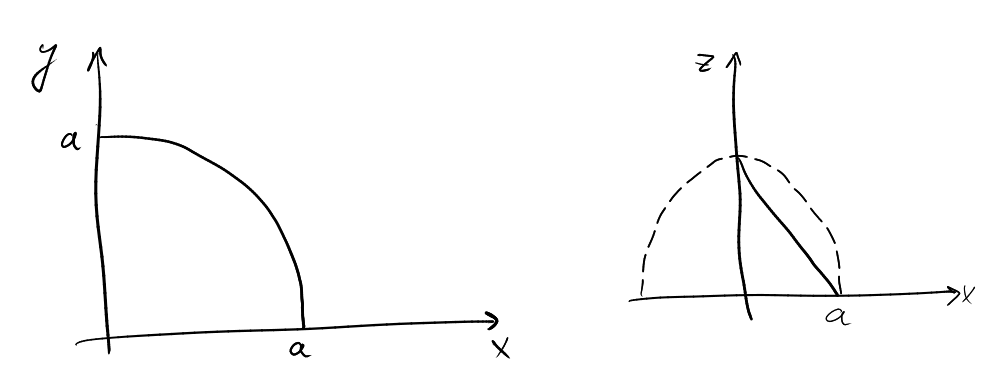
\includegraphics[scale=0.3]{8_2.png}
\end{center}
\[ V = \iiint 1\,dx\,dy\,dz = \iint \,dx\,dy \int\limits_0^{(a^2 - x^2 - y^2)}1\,dz - \iint\dx\,dy \int\limits_0^{a - x - y} 1\,dz = \]
\[ = \int_0^a dr \int_0^{\frac{\pi}{2}} d\varphi \cdpt\frac{a^2 - r^2}{a}\cdot r - \int_0^adx\int\limits_0^{a - x}(a - x - y)\,dy \]
\end{solution}

\begin{task}[4108]
\[ (x^2 + y^2 + z^2)^2 = a^2(x^2 + y^2 - z^2) \]
\end{task}
\begin{solution}
\[ r^4 = a^2(\cos^2\psi - \sin^2\psi)r^2 \]
\[ r = a\sqrt{\cos(2\psi)} \]
\[ V = \iiint_\Omega 1\,dx\,dy\,dz = 2\int_0^{\frac{\pi}{2}} d\psi \int\limits_0^{\sqrt{\cos(2\psi)}}dr \int_0^{2\pi} a^3\cos\psi \cdot r^2d\varphi =  \]
\[ = \frac{4\pi}{3}\int_0^{\frac{\pi}{4}} d\psi \cos\psi\cos^{\frac{3}{2}}(2\psi) \]
\end{solution}

\begin{task}[4121]
\[ (x^2 + y^2 + z^2)^3 = \frac{a^6 z^2}{x^2 + y^2} \]
\end{task}
\begin{solution}
\-
\begin{itemize}
\item \(x = ar\cos\varphi\cos\psi\)
\item \(y = ar\sin\varphi\cos\psi\)
\item \(z = ar\sin\psi\)
\end{itemize}
\[ r^6 = \frac{\sin^2\psi}{\cos^2\psi} \]
\[ r = \sqrt[3]{\tg\psi} \]
\[ V = \iiint 1\,dx\,dy\,dz = 2\int\limits_0^{\frac{\pi}{2}}d\psi\int\limits_0^{\sqrt[3]{\tg\psi}}dr\int\limits_0^{2\pi}a^3 \cos\psi r^2 d\varphi = \]
\[ = \int_0^{\frac{\pi}{2}} \frac{2a^3}{3}\cdot 2\pi \tg\psi \cos\psi\,d\psi = \frac{4a^3\pi}{3} \]
\end{solution}

\begin{task}[4124]
\[ \frac{x}{a} + \frac{y}{b} + \frac{z}{c} = \ln\frac{\frac{x}{a} + \frac{y}{b} + \frac{z}{c}}{\frac{x}{a} + \frac{y}{b}} \]
\[ x = 0,\ z = 0,\ \frac{y}{b} + \frac{z}{c} = 0,\ \frac{x}{a} + \frac{y}{b} + \frac{z}{c} = 1 \]
\end{task}
\begin{solution}
\-
\begin{itemize}
\item \(u = \frac{x}{a}\)
\item \(v = \frac{x}{a} + \frac{y}{b}\)
\item \(w = \frac{x}{a} + \frac{y}{b} + \frac{z}{c}\)
\end{itemize}
\[ J = abc \]
\[ w = \ln \frac{w}{v},\ u = 0,\ w - u = 0,\ w = 1,\ z = 0\leadsto w - v = 0 \]
\[ w = \ln w - \ln v \Rightarrow v = e^{\ln w - w} = \frac{w}{e^w}  \]
\[ V = abc \int_0^1 dw \int_0^w du \int\limits_{we^{-w}}^w 1 dv \]
\end{solution}

\begin{task}[4012]
\end{task}
\begin{solution}
\todo
\end{solution}

\begin{task}[4115]
\end{task}
\begin{solution}
\todo
\end{solution}

\begin{task}[4120]
\end{task}
\begin{solution}
\todo
\end{solution}

\begin{task}[4123]
\end{task}
\begin{solution}
\todo
\end{solution}

\begin{task}[4129]
\end{task}
\begin{solution}
\todo
\end{solution}
\end{document}
